\documentclass{article}
\usepackage[utf8]{inputenc}

% Tables
% Use Roman numerals for tables
% https://tex.stackexchange.com/a/226029
\usepackage[labelsep=period]{caption}
\captionsetup[table]{name=Table}
\renewcommand{\thetable}{\Roman{table}}
% \usepackage{multirow}

\usepackage{pdflscape}
\usepackage{textcomp}
\usepackage{gensymb}

\usepackage{subcaption} % For subfigures?

\usepackage{pifont}
\newcommand{\cmark}{\textcolor{blue}{\textrm{\ding{52}}}}%
\newcommand{\xmark}{\textcolor{red}{\textrm{\ding{56}}}}%

\usepackage{amsmath}
\usepackage{amssymb}

% units
% \SI{X}{\UNIT} will write the value X with units \UNIT. 
% eg. \SI{30}{\celsius}
\usepackage{siunitx} 

\usepackage{graphicx}
\graphicspath{ {./images/} }

\usepackage{todonotes}
\newcommand{\tino}[1]{\todo[inline,color=purple!40]{Tino: #1}}
\newcommand{\fbp}[1]{\todo[inline,color=orange!40]{Ferran: #1}}
\newcommand{\summary}[1]{\todo[inline,caption={},color=yellow!40]{Summary: \\ #1}}

\newcommand{\ssri}[1]{{
\fbox{
\parbox{0.8\textwidth}{  \fbox{$\triangleright$\textcolor{blue}{\textbf{Shashank}:}} 
#1
}}}}

\newcommand{\gbox}[1]{{
\fbox{
\parbox{0.8\textwidth}{  \fbox{$\triangleright$\textcolor{blue}{\textbf{Gon}:}} 
#1
}}}}

\newcommand{\pbox}[1]{{
\fbox{
\parbox{0.8\textwidth}{  \fbox{$\triangleright$\textcolor{blue}{\textbf{From Peter}:}} 
#1
}}}}

\newcommand{\pdebox}[1]{{
\fbox{
\parbox{0.8\textwidth}{  \fbox{$\triangleright$\textcolor{blue}{\textbf{From Philipp}:}} 
#1
}}}}

\newcommand{\editreadybox}[1]{{
\fbox{
\parbox{0.8\textwidth}{  \fbox{$\triangleright$\textcolor{green}{\textbf{READY TO EDIT}:}} 
#1
}}}}

\usepackage[normalem]{ulem}

\setlength{\textheight}{8.4in}
\setlength{\topmargin}{0.1in}
\setlength{\headheight}{0.2in}
\setlength{\headsep}{0.1in}
\setlength{\oddsidemargin}{0in}
\setlength{\textwidth}{6.5in}

\title{``Knees'' in lithium-ion battery aging trajectories}
\author{To do}
\date{}

\begin{document}
\maketitle

**PREVIOUS DRAFT IS NOW IN main\_old\_experiment\_then\_model.tex**

\section{Introduction}

Lithium-ion batteries will continue to play a critical role in decarbonization via their use in electric vehicle and stationary energy storage applications. One of the most challenging requirements for these demanding use cases is long lifetime, with typical warranties of X years for electric vehicles and X years for grid storage[lit values?]. Battery lifetime requirements will only become more demanding as “million-mile batteries” become the expectation for next-generation electric vehicles. Furthermore, as concerns around battery mining, manufacturing, and disposal increase, improving battery lifetime is a straightforward way to reduce the environmental impact of the lithium-ion battery lifecycle. Thus, understanding and improving the lifetime of lithium-ion batteries is a critical research direction.

Lithium ion batteries often exhibit one of three degradation patterns: linear, sublinear, or superlinear aging (Figure \ref{fig:degradation_shapes}). In laboratory settings (i.e., single-cell testing using battery cyclers), degradation is typically presented as capacity, energy, or power vs. cycle number. Cells often degrade linearly[] or sublinearly[]. Sublinear degradation is often attributed to side reactions such as the solid-electrolyte interphase (SEI) growth, which grows approximately[] (but not exactly[]) with the square root of time or cycle number due to its self-passivsting nature. While this type of degradation is largely unavoidable, the decelerating degradation rate is a fortunate property for long-lifetime applications. However, superlinear battery degradation is also observed (Figure \ref{fig:degradation_shapes}c). This type of degradation goes by many names in the battery literature, including ``knee'', ``rollover failure'', ``sudden death'', ``accelerated aging'', ``nonlinear aging'', ``saturation'', etc; we use the term ``knee'' in the remainder of this work. Avoiding knees is critical to ensure long lifetimes. However, despite many experimental and modeling reports on this topic, a comprehensive understanding of knees is lacking due to the variety and complexity of the proposed mechanisms.


\begin{figure}[ht]
\centering
\includegraphics[scale=1]{figures/degradation_rates.eps}
\caption{The three lithium-ion battery aging trends observed in the literature: sublinear, linear, and superlinear degradation (``knees''). Knees are incompatible with long battery lifetimes. Here, the x axis is labeled ``cycle number'', although it could also represent equivalent cycles or similar; similarly, the y axis is labeled ``capacity'', although it could also represent energy or power. We use this convention (``capacity vs. cycle number'') in conceptual figures throughout this work.}
\label{fig:degradation_shapes}
\end{figure}


In this review, we survey the literature and critically examine both experimental and modeling work on the subject of knees. We first review methods to define the knee point. We then identify (five/six) knee ``pathways'' from the literature, including lithium plating, resistance growth, additive depletion, percolation-limited connectivity, and mechanical deformation. We also classify differences in experimentally observed knee behavior as either differences in design, differences in usage conditions, or cell-to-cell/testing variation. Finally, we discuss the implications of our review to both predicting and avoiding knees, and we suggest future work on this topic. This review can serve both academic and industrial efforts to understand and improve battery lifetime.

\newpage
\section{Defining the knee point}

\editreadybox{}

\pbox{
Key messages in my mind:
\begin{itemize}
    \item Knees seem easy to identify by eye, and have a nice mathematical description as the second derivative
    \item However noise makes this nontrivial (figure)
    \item No formal definition (IEEE standard)
    \item Briefly describe different methods
        \subitem SG: We don't want this to take up too much space. If possible, a single plot with diagrams should suffice.
\end{itemize}
}

While the \textit{presence} of a knee is generally straightforward to identify, the \textit{location} of a knee is less so.
Mathematically, the knee is described as the point at which the degradation rate is changing fastest, i.e., the second derivative reaches some maximal value.
Furthermore, locating a knee by eye is seemingly straightforward for a single, smooth and ideal aging profile (e.g.\, the superlinear aging trend in Figure \ref{fig:degradation_shapes}).
However, both of these approaches are challenging when the aging profiles exhibit noise (often due to thermal fluctuations). Figure \ref{fig:knee_definition3} displays...(Sam to complete using text below)
However, that point appeared slightly after where we put the knee, and Figure \ref{fig:knee_definition3} demonstrated how even small amounts of noise ($\sigma=0.05\%$ capacity) cause significant issues. Consequently, we concluded that health metric profiles should be smoothed prior to knee identification.

\begin{figure}[ht]
\centering
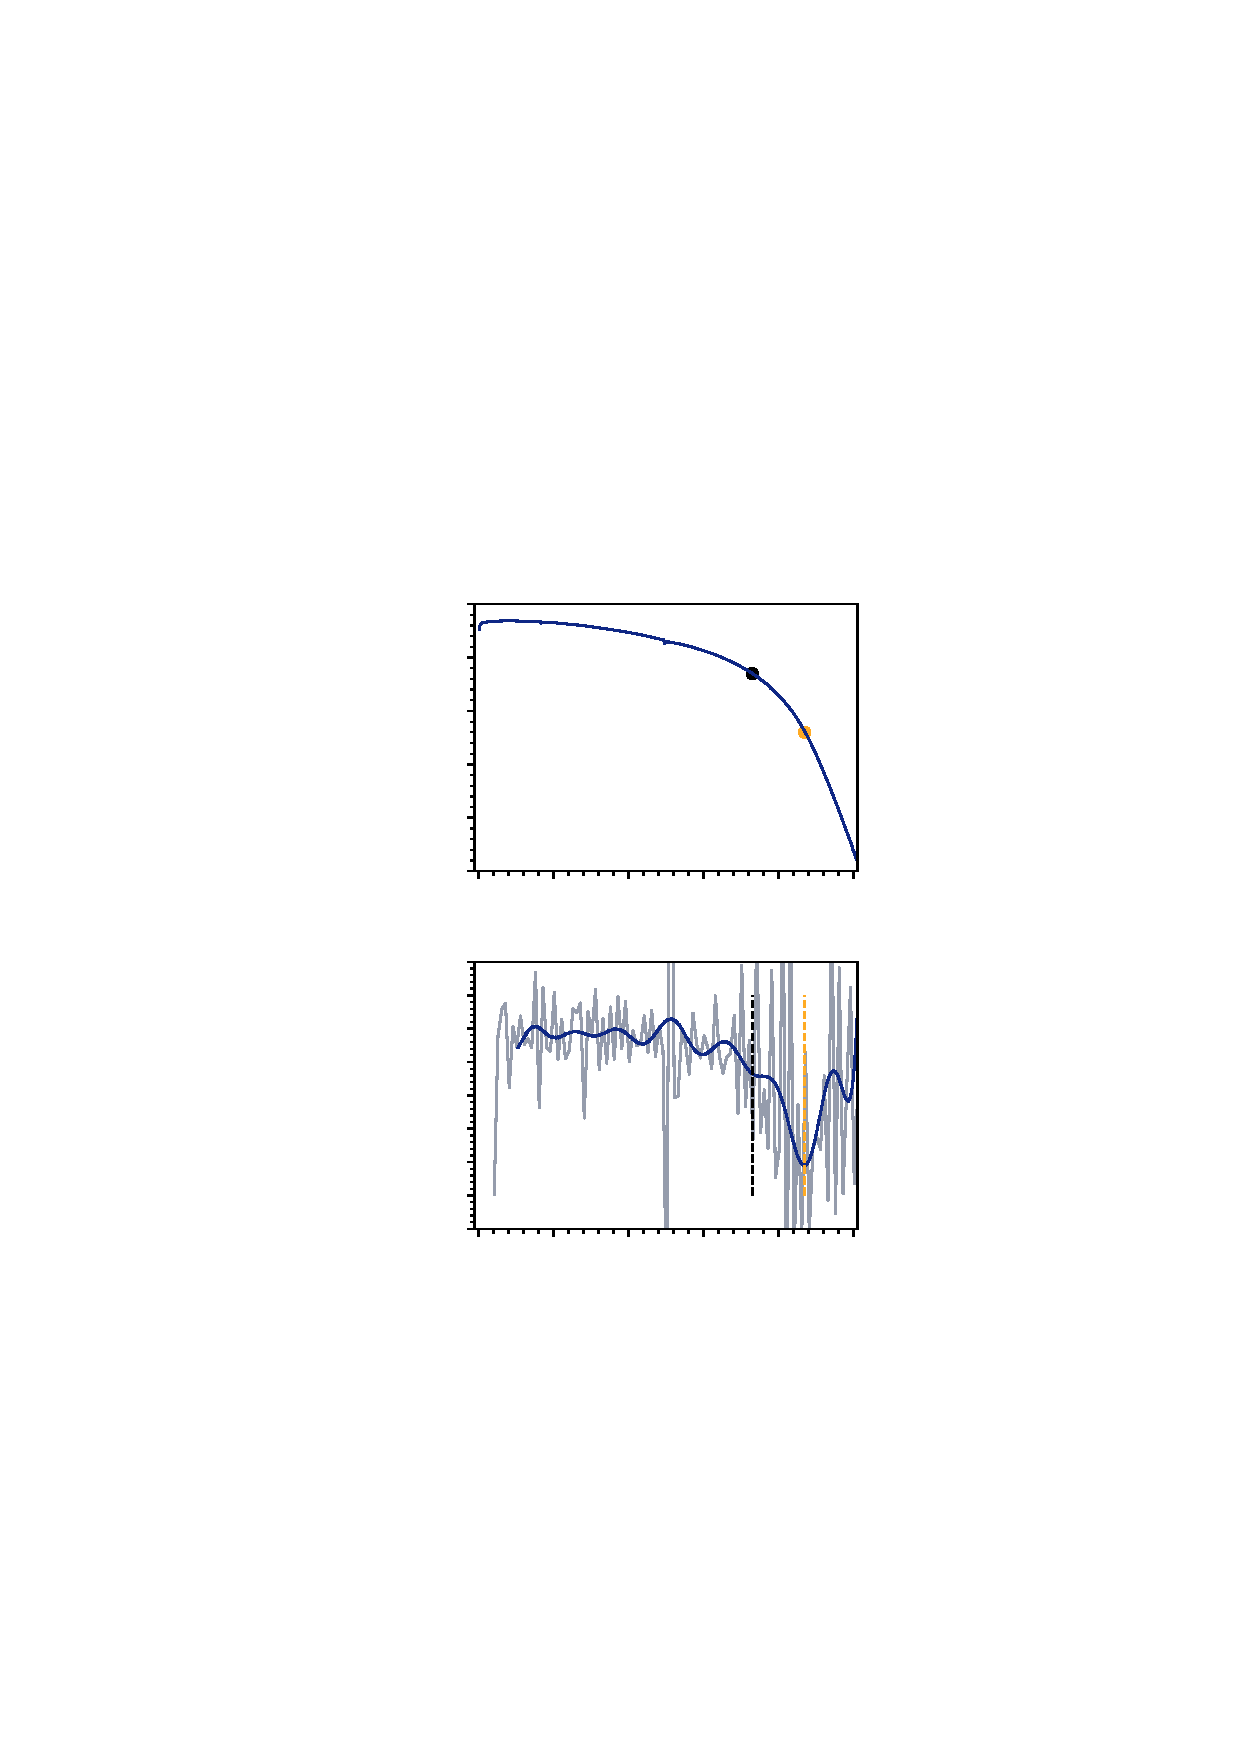
\includegraphics[width=\textwidth]{images/knee_definition.pdf}
\caption{Definition of a knee point. (Sam to complete caption). Also please label the panels with a and b, replace "cycles" with "Cycle number", and make x axes the same scale) [SG: the "cycles" is a count of throughput, not the "cycle number". I can easily change the data if preferred]}
\label{fig:knee_definition3}
\end{figure}

Several knee point identification methods have been proposed in the literature. IEEE Standard 485\texttrademark-2010  \cite{noauthor_ieee_2011} defines a knee as a change to a stage of rapid decrease in capacity. However, this definition is qualitative and thus hard to practically apply.

\begin{figure}[ht]
\centering
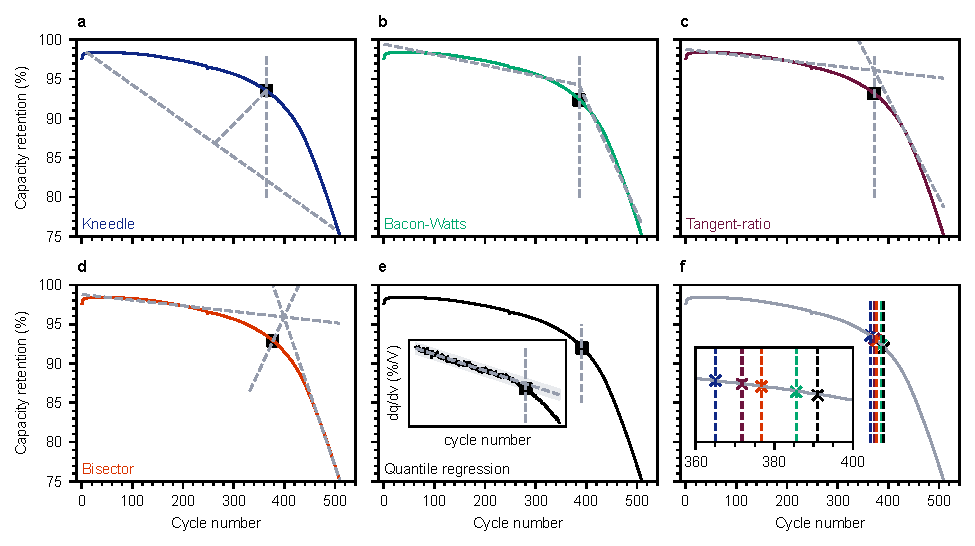
\includegraphics[width=\textwidth]{images/knee_identification_methods.pdf}
\caption{Different knee identification methods exemplified on Data from \cite{severson_data-driven_2019} cell of batch 2, channel 12. (a) Bacon-Watts \cite{fermin-cueto_identification_2020}, (b) Kneedle \cite{satopaa_finding_2011}, (c) Diao et al.~\cite{diao_algorithm_2019}, (d) Zhang et al.~\cite{zhang_identifying_2020}, (e) bissector and (f) comparison. 
{\color{blue} Data from \cite{severson_data-driven_2019}, batch 2, channel 12.} (Nice work! Sam to add caption and panel labels {\color{green} Labels added. Do you want these as distinct images with descriptions under each? }. Try tight layout? 
% Also include the second derivative here? what dataset is this cell from?\cmark )
WAIT UNTIL END TO ADD CITATIONS IN THE TEXT}
\label{fig:knee_identification_methods}
\end{figure}


(Sam -- looking good, but please add a brief in-text discussion of the figure).


Kneedle is an example of a quantitative approach. It calculates the knee as the point of maximum curvature of the capacity curve \cite{satopaa_finding_2011}. The knee can be calculated using a Bacon-Watts method for estimating the transition between two intersecting lines fitted to a capacity fade curve, a method which can also provide an estimate of ``knee-onset'' \cite{fermin-cueto_identification_2020}. Other methods use tangential lines to define the knee based on characteristic points of the capacity curve \cite{diao_algorithm_2019} and linear extrapolations of early and late life, the latter is shown in Figure \ref{fig:knee_definition} as an example of robustness to noise CITE.

Finding the knee online, i.e.\ during use, is difficult because there is no knowledge of the end of life capacity profile. One method found was to approximate early life with a linear regression then define a cell to have met the knee when the capacity leaves a defined region about that regression \cite{zhang_accelerated_2019}.

These methods were implemented and tested in database of \cite{severson_data-driven_2019} to assess consistency. Kneedle consistently identified a knee point prior to that of Bacon-Watts, but in general they all achieved a similar performance even if that performance could only be defined relative to one another without any known ground-truth.
\gbox{do we add the linear regressions to supplementary material?}


\gbox{
Plan for the section (identify the references):
\begin{itemize}
    \item The IEEE Standard 485\texttrademark-2010 \cite{noauthor_ieee_2011}\cmark 
    % relates the “knee” with the transition to a stage of rapid decrease in capacity. This definition is qualitative not quantitative.

    \item Very brief Overview of methods 

    
    \begin{itemize}
        \item \cite{fermin-cueto_identification_2020}\cmark 
        % , define the Knee based on Bacon Watts method for estimating the transition between two intersecting lines fitted to the capacity fade curve. Has the advantage of providing the concept of knee-onset.
        \item Kneedle  \cite{satopaa_finding_2011} \cmark 
        % , define the knee as the point of maximum curvature of the capacity curve
        \item Diao \cite{diao_algorithm_2019}, define the knee as the intersection of two tangent lines to the capacity fade curve drawn at two significant points (an inflection point and the point of maximum slope changing ratio)
        \item \cite{zhang_accelerated_2019} quantile, defined the knee-point as the intersection of two straight lines with different slopes and proposed an algorithm for online knee detection based on quantile regression (some parameter tuning is required). They fit a median regressor to the State of Health data and they define the knee as the first point at which the SOH data is outside a safety zone around the median regression line.
        \item {\tt Sam's Bissector}  
    \end{itemize}
    
    These methods we implemented, and (empirically) tested in database of \cite{severson_data-driven_2019}. Noteworthy of remark is that the Kneedle's knee was always ahead of the Bacon Watts knee. In view of the a linear regression analysis between knee-point to EOL, 
    
    \item Present empirical analysis plot of linear regressions across datasets for knee-2-EoL (?) Supplementary material?
    \end{itemize}
}


%%%%%%%%%%%%%%%%%%%%%%%%%%%%%%%%%%%%%%%%%%%%%%%%%%%%
%%%%%%%%%%%%%%%%%%%%%%%%%%%%%%%%%%%%%%%%%%%%%%%%%%%%
%%%%%%%%%%%%%%%%%%%%%%%%%%%%%%%%%%%%%%%%%%%%%%%%%%%%
%%%%%%%%%%%%%%%%%%%%%%%%%%%%%%%%%%%%%%%%%%%%%%%%%%%%


\section{Pathways for knee points}

We surveyed the literature and identified six pathways for knees to occur. These pathways are schematically illustrated in Figure X. Some of these pathways (e.g., lithium plating) have been extensively characterized and modeled, while others (e.g., percolation-limited knees) are merely hypotheses. Here, we critically examine the evidence for each pathway. For more extensively studied pathways such as lithium plating, we consider both \textit{modes}, defined as high-level changes in cell state, and \textit{mechanisms}, defined as the specific failure that leads to a change in cell state. For instance, active material loss is a degradation mode that can be caused by electrode delamination, a failure mechanism. While failure mechanisms are often challenging to pinpoint exactly, failure modes can be considered to conceptually validate a proposed pathway.

We also consider the relationship between the observable state variables (i.e., capacity, energy, and power) and the mechanisms underlying their knee points. Figure \ref{fig:snowball_vs_hidden_vs_threshold} illustrates three underlying mechanisms that can lead to a knee. ``Snowball'' mechanisms (Figure \ref{fig:snowball_vs_hidden_vs_threshold}a \& d) occur when the underlying state variable has a direct relationship with the observable state variable, but the underlying state variable is exponentially increasing. ``Hidden'' mechanisms (Figure \ref{fig:snowball_vs_hidden_vs_threshold}b \& e) occur when the observable state variable, originally controlled by a slowly-increasing state variable, becomes dominated by a second rapidly-increasing state variable. Finally, ``threshold'' mechanisms (Figure \ref{fig:snowball_vs_hidden_vs_threshold}c \& f) occur when the observable state variable changes when the underlying state variable reaches a threshold. Each of these underlying mechanisms has unique implications for detectability and prediction, a point we return to throughout this work.

\begin{figure}
    \centering
    \includegraphics[width=0.7\linewidth]{figures/snowball_vs_hidden_mechanism.eps}
    \caption{Different types of underlying mechanisms leading to a knee. In each case, the retention curve looks the same (a-c), but the underlying mechanism has a different functional form. (d) ``Snowball'' mechanism, in which the state variable is exponentially increasing. (e) ``Hidden'' mechanism, in which a slowly-increasing state variable is dominated by a rapidly-increasing state variable. (f) ``Threshold'' mechanism, in which a dramatic change in observable state is triggered by a state variable reaching a threshold.}
    \label{fig:snowball_vs_hidden_vs_threshold}
\end{figure}

\subsection{Lithium plating}

\pbox{
Plating to do's:
\begin{itemize}
    \item General intro to plating
    \item Cartoon for all plating modes
    \item Figures
    \item Editing (Peter)
\end{itemize}
}

Lithium plating occurs when lithium ions form metallic lithium on the surface of the electrode rather than intercalating into it. The plating reaction becomes favorable when the equilibrium potential of Li/Li+ is greater than the equilibrium potential for other alternative reaction pathways for Li+.\ref{plate} Many pathways for plating exist, and they can be broken into two categories. Thermodynamic plating can be defined as plating which is not heavily influenced by current. These pathways occur when the $V_{anode}$ term in equation \ref{plate} approaches 0 V against Li/Li+ as a result of temperature\cite{wang_pnas} or as a result of the electrode approaching its lithium capacity. Kinetic plating occurs when current-induced conditions cause $\eta_{plating}$ to drop below 0 V against Li/Li+. Typically, this means $\eta_{anode}$ is very low, however, large concentration gradients caused by high current in conditions which lower the diffusion coefficient (such as fast charging under cold ambient temperature) can cause $V_{anode}$ to drop locally. Since lithium plating can lead to irreversible and rapid loss of lithium inventory, it is one of important mechanisms to study in the context of kneepoints. The remainder of this section enumerates the pathways by which plating can lead to a kneepoint. 

\begin{equation}
    \eta_{plating} = V_{anode}+\eta_{anode}-V_{plating}+R_{SEI}I
    \label{plate}
\end{equation}






Intro to plating
\begin{itemize}
    \item What is Li Plating?
    \item Why does plating occur generally (V<Li)
    equilibrium potential of the Li$\mathrm{^0}$/Li$\mathrm{^+}$ > everything else
    \item Brief introduction to and definition of each plating pathway
    \subitem Thermodynamic "non-current-induced"
    \subitem Kinetic "current induced"
\end{itemize}

\subsection{Thermodynamic Lithium Plating}

- x$>0$
- heterogeneous temperature
- ${LAM}_{de}$NE

\subsubsection{$\textbf{LAM}_{de}$NE}

\pbox{READY FOR EDITING}

Loss of active material of NE for lithium insertion is caused mainly due to particle cracking and electrical contact loss/blockage of active sites by resistive surfaces. Lithium trapped inside isolated graphite particles can contribute to cell capacity decrease due to unavailability to cycle. K.Jalkanen et al \cite{jalkanen_cycle_2015} showcased cyclic aging at different cycling temperatures (\SI{25}{\celsius}, \SI{45}{\celsius} charge and \SI{65}{\celsius} discharge) through capacity fade. At temperatures above \SI{60}{\celsius}, aging at NE (graphite electrodes) is different compared to low temperature aging. Elevated temperatures contribute to excess Li plating during  cycling apart from the SEI-layer increase on anode surface which occurs during normal charging and discharging cycles at room temperature. Increase in SEI-layer thickness enhances graphite electrode polarization leading to additional plating. SEI-growth also leads to electrolyte consumption due to prolonged cycling at high temperatures. Irreversible lithium plating reduces graphite electrical contact, when lost, results in isolated dead lithium and capacity degradation \cite{petzl_lithium_2015}.  
Dubarry et al \cite{dubarry_durability_2018} modeled LAM and LLI and showed that a knee occurs if LAM NE is faster than LLI, with faster knee onset for higher LAMne:LLI ratios. The impact of gassing and dry-out has been modeled by Kupper et al \cite{kupper_end--life_2018}.

Localized loss of negative electrode active material sites can cause heterogeneous Li plating by impeding the transport of Li, locally increasing the over-potential and eventually causing plating. There are several mechanisms that may lead to LAMdeNE: surface layer growth, delamination, and electrolyte dry-out. 
Electrode sites may become inaccessible due to electrolyte dry-out. Electrolyte dry-out occurs in electrolyte lean cells due to decomposition of the electrolyte into gas and eventual de-wetting, causing some of the electrode to become inaccessible; cell gassing and dry-out often occurs in parallel with other degradation modes, and is thus difficult to deconvolute from other degradation modes during cycle aging. However, several calendar aging experiments have been conducted to investigate gassing and electrolyte dry-out impacts on cell performance. Mao et al clearly demonstrated the impact of dry-out during calendar aging at high temperatures, connecting accelerated capacity fade to gassing and electrolyte dry-out \cite{mao_calendar_2017}. They also determined that a small stack pressure of about 4 PSI mitigates the occurrence of dry-out within the porous electrodes due to gas formation by displacing gasses to the edges of the cell pouch. Xiong et al studied the impact of storage potential, temperature, and electrolyte composition on the volume and composition of gasses generated by electrolyte decomposition, finding that not only does electrolyte composition play a major role, but also that interactions between species generated separately at the anode and cathode is responsible for the decomposition of the electrolyte \cite{xiong_studies_2017}.

Surface layer growth on the negative electrode may impede Li transport into the negative electrode during charging. This surface layer has been often observed during accelerated aging of LIBs, and is most commonly attributed to Mn or Fe dissolution from the cathode and electrolyte salt decomposition \cite{lewerenz_post-mortem_2017,lewerenz_systematic_2017,zhu_investigation_2021,stiaszny_electrochemical_2014,rahe_nanoscale_2019,keil_linear_2019,sarasketa-zabala_understanding_2015, willenberg_high-precision_2020}. Lewerenz et al documented surface layer growth very thoroughly, finding that increasing C-rate and larger depth-of-discharge could lead to earlier onset of a knee, which was correlated with the presence of a thick surface layer on cells that contained knees; cells without knees also contained obvious surface layers, but with lower surface coverage and less thickness \cite{lewerenz_post-mortem_2017,lewerenz_systematic_2017}. These surface layers sometimes seem to lead directly to localized lithium plating, with lithium observed on top of the layer \cite{zhu_investigation_2021}. Delamination may also lead to inaccessible negative electrode material, which can potentially cause lithium plating and knee-onset. Willenberg et al conclusively observed delamination induced knee-onset in cylindrical cells; delamination was caused due to mechanical stresses and deformation after the formation of a surface layer on the negative electrode \cite{willenberg_high-precision_2020}. Cannarella et. al. also observed surface layer growth and delamination as a function of stack pressure in multi-layer pouch cells \cite{cannarella_stress_2014}. Pfrang et al observed delamination in cylindrical cells, though sometimes without observing knee-onset \cite{pfrang_long-term_2018}.

\subsection{Kinetic Plating}
%- this is when transient effects cause plating
%    - Low T -> Low D -> High Surface x -> ${eta}_{s}$<0
%    - Low OCV + High ${eta}_{op}$ -> ${eta}_{n}$<Li
%    - High σ -> Low ρ -> High Surface x -> ${eta}_{s}$<0
 %   - SEI -> Low ρ -> High Surface x ->${eta}_{s}$<0

\subsubsection{Direct Thermodynamic Lithium Plating MOVE}

\pbox{READY FOR EDITING}

Li inventory loss due to thermodynamic Li plating may occur whenever there is not enough negative electrode capacity to store all of the available lithium during charging.  This well-known plating mode has been used intentionally by several researchers.  Martin et al [1] used deposited Li metal as a mechanism to store extra capacity, enabling the cell to occasionally discharge extra energy without requiring a larger anode,effectively increasing the specific volumetric energy density of the cell. Single crystal NMC pouch cell with n:p value of 0.6 was used as a hybrid anode (conventional graphite and graphite/ lithium metal). Three different electrolytes (2F1L, 2VC and LDBF) were utilized for cycling evaluation. High upper cutoff voltage cycling showcased the plating effect on the different electrolytes and was the primary failure mechanism with over 50\% capacity loss of lithium metal in 2F1L and 2VC.  
\begin{figure}
\centering
\includegraphics[scale = 0.4]{images/Differential Capacity vs Voltage.jpg}
\caption{Differential Capacity vs Voltage for 0.75 n:p and 0.5 n:p.}
\label{fig:DiffCapVoltageNP}
\end{figure}
Researchers at Sandia National Lab also created cells with limited negative electrode capacity (N:P ratios of 0.75 and 0.5) to intentionally deposit Li metal to study the failure behavior of cells after Li plating has occurred [2]. Deichmann et al [2] experiments for coin and pouch cells indicated a relationship between decreased n:p and capacity fade at high cycle number during cell cycling. Loss of Lithium inventory is attributed the leading cause for capacity fade. Differential capacity plots in Figure 3b present a comparison between the 0.75 n:p and 0.5 n:p coin and pouch cells, with charge and discharge amplitudes decreasing at high cycle number indicating reduced cell capacity caused due to loss of lithium inventory during deposition of Lithium. Morphological changes were observed in SEM analysis with the 0.75 n:p anode imaging demonstrating an increase in amount of Li deposition on graphite surface, while 0.5 n:p anode imaging shows intertwined dendrites spanning entire graphite electrode. 

\subsubsection{Direct Kinetic Lithium Plating}
Li plating may also occur when the local Li+ potential exceeds the nucleation barrier leading to direct plating, this could occur at electrodes potentials greater than zero (vs. Li/Li$\mathrm{^+}$). Direct heterogeneous Li plating can be driven by a wide range of design and usage conditions; the typical usage case leading to Li plating is high charging rates at low temperature \cite{waldmann_temperature_2014, petzl_lithium_2015}. Waldmann et al.,\cite{waldmann_temperature_2014} observed an increase in the rate of ageing with a decrease in temperature below 25$\circ$C and attributed the increasing in rate of ageing to lithium plating. At low temperatures, lithium ions have less energy to cross the potential barrier on SEI and in graphite electrodes. This low temperature plating was validated by experiments on 18650 pouch cells of LNMC and LMO blends and graphite anode. Note that there are no consistent quantitative values for ‘high’ charging rate or ‘low’ temperature, as plating will occur whenever the local potential exceeds the energy barrier for Li nucleation. Thus, plating may be observed even at fairly normal test conditions, such as 1C CC charging near room temperature \cite{waldmann_optimization_2015,burns_-situ_2015}. Increasing temperature and cell design may allow for much more rapid charging before Li plating and knee-over is observed; Lewerenz et al cycled cells at rates up to 8C, observing no obvious knee-over up to 4C, though microstructural evidence of Li plating was found even at 1C \cite{lewerenz_systematic_2017}. The onset of direct lithium plating is also very sensitive to the charging protocol, with many studies demonstrating that informed design of charge protocols can substantially extend cell lifetime by preventing direct lithium plating \cite{waldmann_optimization_2015,schindler_fast_2018}.

Mechanical stress on the cell pouch or cell casing may also lead to direct kinetic lithium plating, as applied stress can compress the electrode. This reduces the porosity of the electrodes in a small region, reducing the diffusivity of electrolyte and thus increasing the local polarization and potentially causing lithium plating. A direct test of this cause was conducted by Liu and Arnold \cite{liu_effects_2020}, who demonstrated that localized lithium plating could be controlled by densifying regions of the separator, which decreases the local lithium diffusivity and led to localized lithium plating. Many examples exist mechanical stress leading to lithium plating, as well. For example, Bach et al applied a hose clamp around the circumference of an 18650 cell, and a post-test tear down clearly showed lithium plating localized to regions of the electrodes that were under compressive stress \cite{bach_nonlinear_2016}. Pouch format cells also show similar results. Fuchs et al \cite{fuchs_post-mortem_2019} applied pressure using a metal bearing. Liu et applied pressure to electrodes in a coin cell setup using various shapes, producing legible shapes and letters using localized lithium plating \cite{liu_size_2018}.
Check also Okasinki https://pubs.rsc.org/en/content/articlepdf/2020/cp/d0cp04436a

\subsubsection{Pore clogging}
As SEI forms, it precipitates mainly in the pores of the anode, causing reductions in the volume fraction of the electrolyte in the anode (Sikha, 2004). The decreased volume fraction causes increased over-potential, ultimately leading to increased plating. The plating also helps to reduce the volume fraction, thus creating a positive feedback loop which accelerates aging(cite Yang 2017). This phenomenon also causes a voltage undershoot, particularly noticeable at high discharge rates (3C) (cite Yang 2017). Several authors have noted that a critical porosity exists around 0.05, and pore clogging beyond that induces the period of accelerated aging (cite Yang 2017, Muller, 2019). Additionally, some authors model the same effect by changing the diffusion coefficient as a function of cycle number (Keil, 2020). One possible mitigation for this issue is to use a graded or stepped porosity profile. Since most pore clogging occurs near the separator, having a higher porosity near the separator and a lower porosity near the current collector helps to slow the onset of the accelerated aging caused by pore clogging (Muller, 2019).
\subsubsection{Others}

\begin{figure}[ht]
\centering
\includegraphics[scale = 0.7]{images/Capacity & Diff Voltage.png}
\caption{Capacity and Differential Capacity vs Cycle number.}
\label{fig:CapDiffCapCycle}
\end{figure}

Apart from the main mechanisms causing knees due to plating, few other causes are based on substantial and mild temporally thermal transient conditions lead to a rapid capacity fade in cells when compared with cells at a fixed equilibrium temperature. Temporal transient thermal gradients (40 \degree C to 0 \degree C) contribute to Li ions being plated as Li instead of intercalating, which accelerates capacity fade over subsequent cycles causing knees and ultimately resulting in jellyroll collapse.
Equilibrium cells at 40 \degree C, 20 \degree C, 0\degree C and transient cells (40\degree C to 0 \degree C and 10 \degree C to 0 \degree C) are tested for understanding of the thermo-electrochemical coupling across different temperature (Carter 2019).Differential voltage from charging gives route to plating detection and discharging cycle showcases the degradation modes. Equilibrium cells at 40 \degree C and 20 \degree C show minimal degradation while equilibrium cell at 0 \degree C has initial minimal degradation, then a gradual decay midway. On the contrary, transient 10 \degree C to 0 \degree C cell and 40 \degree C to 0 \degree C cell show degradation at earlier cycles (8 and 5 respectively) (Carta, 2019). Transient 40 \degree C to 0 \degree C cell demonstrates high lithium stripping during initial discharge cycles due to thermal transient induced plating causing increase in anode thickness, pressure buildup in jelly role and capacity loss. The decrease in differential voltage for transient cells immediately with the start of the cycle shows the degradation evidence by lithium plating.  Figure \ref{fig:knee_definition} highlights the difference between the 0 \degree C and Transient 40 \degree C to 0 \degree C jellyroll collapsing behaviors. Primary reason for degradation is jellyroll collapse for 0 \degree C cell while the rapid lithium plating followed by jellyroll collapse causes capacity fade knee point in Transient 40 \degree C to 0 \degree C cell. 


\subsection{DCR growth}


\pbox{
One way to organize this section would be:
\begin{itemize}
    \item Intro to the phenomenon: Electrolyte oxidation on positive electrode well known to cause DCR growth. 
    \item Cells have different V-Q curves; generally, flat part at high SOC and steep part at low SOC
    \item Discuss figure, explain how this is a threshold mechanism. Understand/discuss capacity vs energy vs power knees (the power knees are pretty strange)
    \item Cell design factors that exacerbate DCR growth: uncoated cathodes, methyl acetate, low salt concentration (all from Ma et al.). Cathode chemistries like LFP have a flatter voltage curve and thus will severely experience this effect
    \item Cell usage factors that exacerbate DCR growth: High upper cutoff voltage / time at high SOC, high temp
    \item Secondary effects (feedback loop between high DCR -> high temperature -> lower DCR). Not sure if this is worth discussing
    \item Table summarizing each paper - table variables: capacity at knee onset, resistance at elbow onset, EOL capacity, EOL resistance
    \end{itemize}
}

Summary: DCR resistance affects when you hit your cutoff voltage during charging and discharging. DCR resistance itself is a function both of cell state-of-health as well as cell temperature. Increased DCR resistance will then also lead to increased heat generation during the flow of current, which can lower resistance as more current is passed over the cell; this may lead to different results depending on cell architecture (coin, cylinder, pouch, prismatic) and cooling. And of course, you can test at different cutoff voltages.

Increasing DC resistance during cycling may also lead to the onset of not only a knee in cell power but also in the accessible capacity. This is intuitive at high currents, when the cell may hit a voltage limit before the majority of lithium has been shuttled across the separator, leading to a lower measured capacity. However, during aging, this rate limitation may occur at much lower than expected C-rates, and appear as a knee in the plots of power and capacity versus cycles. This behavior was thoroughly studied by Ma et al \cite{ma_editors_2019} using lab-made 230mAh NMC532/graphite pouch cells, varying electrolyte composition as well as the type of graphite. Careful study using impedance measurements, both of the full cells as well as symmetric coin cells of the positive and negative electrodes, was used to isolate the loss of performance to a dramatic increase of the cathode impedance during aging. This DC resistance growth was attributed to electrolyte oxidation at the positive electrode, which varied according to the upper cutoff potential as well as the electrolyte composition. Similar onset of a capacity knee due to the selection of the electrolyte composition was previously observed by Li et al as well (Li et al 2018 Methyl acetate.. In Zotero but not here). 

Many other researchers have observed substantial DC resistance growth correlated with knee onset. A detailed aging study by Ecker et al \cite{ecker_calendar_2014} observed capacity knee onset correlated with dramatically increased DC pulse resistance (100-300 percent increase from beginning of life) when cycling 2 Ah NMC/Gr 18650 cells at 1C constant current at 30C, as well as when calendar aging at 100 percent SOC and 50C. Rahe et al \cite{rahe_nanoscale_2019} observed a 3.6x increase in DC pulse resistance before reaching 80 percent remaining capacity when cycling 40 Ah NMC111/Gr pouch cells at 2C constant current, observing substantial cathode particle cracking and cathode current collector oxidation. Willenberg et al \cite{willenberg_development_2020} observed an approx. 100 percent increase in DC pulse resistance correlated with the capacity knee onset and a near total loss of available capacity after cycling 3.35 Ah NCA/Gr+Si Samsung SDI 35E cells at only 10 percent average state-of-charge and 20 percent depth of discharge under 0.5C constant current. Broussely et al \cite{broussely_main_2005} observed 100-400 percent increase of 5s DC pulse resistance correlated to a knee onset at about 70 percent remaining capacity in 1.3 Ah LCO/Gr pouch cells cycling at 100 percent depth-of-discharge with 1C and C/2 constant current charging and discharging, respectively. Schuster et al \cite{schuster_nonlinear_2015} observed a 200 percent increase in cell impedance at 50 percent state-of-charge after knee onset at about 80 percent remaining capacity when aging 1.95 Ah NMC/Gr 18650 cells from Molicel at 25 C using 1C and 2C constant current charging and discharging, respectively. Schuster et al used impedance analysis to separate the overall impedance increase into a 40 percent increase to Ohmic resistance and a 400-500 percent increase to charge transfer resistance. Post-mortem characterization revealed the existence of the formation of a resistive surface film at the anode/separator interface in cells which experienced a capacity knee. Lewerenz et al \cite{lewerenz_systematic_2017, lewerenz_post-mortem_2017} observed high correlation of capacity knee onset to the appearance of the onset of rapid growth of the DC pulse resistance when aging cylindrical 8 Ah LFP/Gr cells at 40 C and at various C-rates and depths-of-discharge. In this study, many cells were aged, and capacity knees were only observed in cases where accelerated resistance growth was also observed; several cells experienced substantial capacity loss (40-50 percent loss) and resistance growth (30-50 percent), but without any dramatic increase in the capacity loss or resistance growth rates during aging. The appearance of a knee was correlated to the presence of a resistive covering layer at the anode/separator interface, which covered approximately the center third of the anode \cite{lewerenz_post-mortem_2017}. Martinez-Laserna et al \cite{martinez-laserna_technical_2018} observed a few examples of a capacity knee onset at about 80 percent remaining capacity associated with accelerated an resistance growth with between 100-400 percent increased resistance when aging 20 Ah NMC/Gr through both a first life and a second life, with various aging conditions and cell states at the end of first life as well as the end of second life. This work also demonstrated a counterexample to some of the prior works, however, with several cells experiencing a acceleration of their resistance growth resulting in about 100-200 percent resistance growth without an observable capacity knee. Braco et al \cite{braco_experimental_2020} observed a correlation between the accelerated resistance growth and capacity knee onset in Nissan Leaf EV LMO/Gr cells aging under 1C constant current at 25 C, measuring 300-400 percent resistance growth starting at approx. 65 percent remaining capacity. Frisco et al \cite{frisco_understanding_2016} observed capacity knee onset at about 80 percent remaining capacity correlated with 400 percent increased DC resistance when aging Samsung NCA/Gr cells when cycling at approx. C/3 constant current charge and discharge at room temperature.  Klett et al \cite{klett_non-uniform_2014} observed the onset of a capacity knee at about 80 percent remaining capacity correlated with onset of accelerated resistance growth, leading to about 100 percent resistance increase and a capacity loss from 80 percent to 30 percent when aging 2.3 Ah LFP/Gr 26650 cylindrical cells using dynamic drive cycles at room temperature. Pfrang et al \cite{pfrang_long-term_2018} observed a capacity knee at about 75 percent remaining capacity correlated to accelerated resistance growth onset at about 40 percent increased resistance when aging Sanyo UR18650E NMC/Gr cells at 33 C using 1C constant current cycling at various average states-of-charge and depths-of-discharge. Wunsch et al \cite{wunsch_investigation_2019} observed capacity knee onsets at relative capacities as high as 97 percent, correlated to the onset of accelerated resistance growth onset even before any resistance growth has occurred, while also observing substantial capacity loss and resistance growth without any acceleration effects.

\begin{figure}[]
\centering
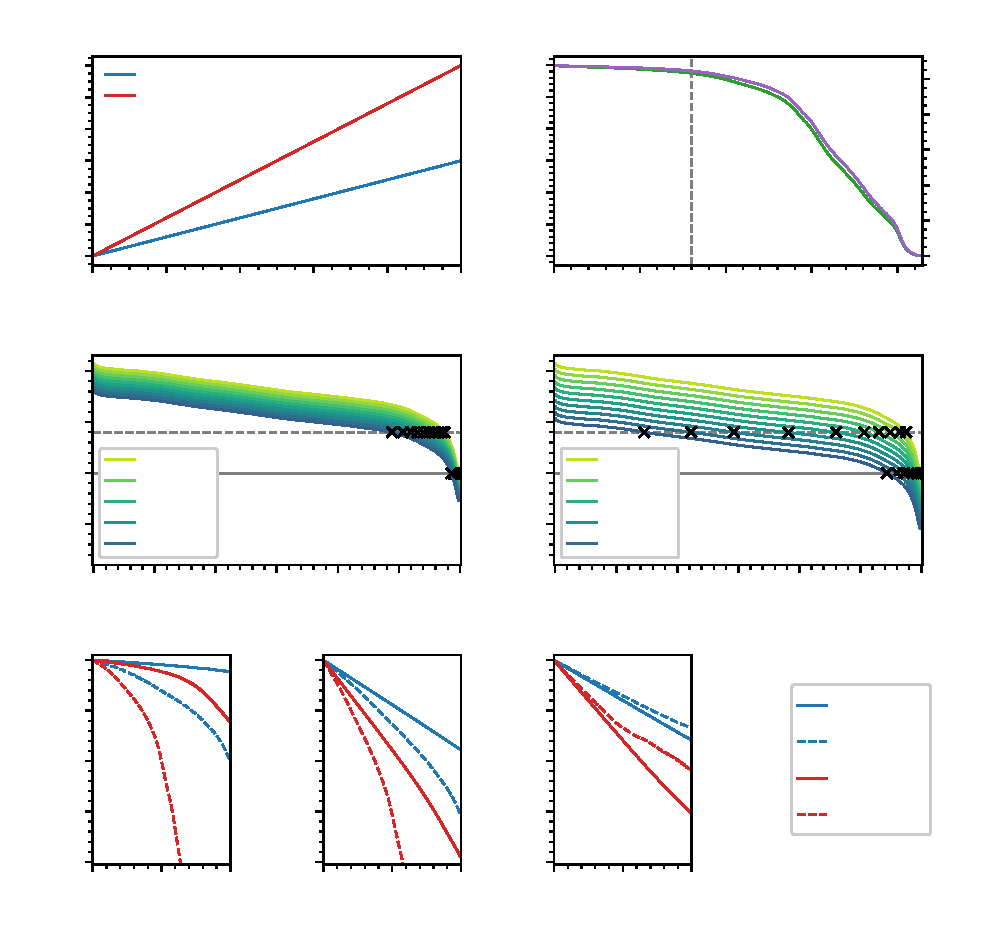
\includegraphics[scale = 0.9]{figures/dcr_growth_knee_2.eps}
\caption{Simple model illustrating ``pseudo-knees'' due to DCR growth. Inspired by Figure 16 of Ma et al.\cite{ma_editors_2019} and Mandli et al.\cite{mandli_analysis_2019}. (a) Assumed overpotential growth vs. cycle number for a 1C and 2C discharge. The assumed DCR growth rate is 0.2 m$\Omega$/cycle. (b) Discharge capacity and energy vs. the minimum discharge voltage. (c, d) Voltage vs. capacity as a function of cycle number for the (c) 1C discharge and (d) 2C discharge cases. The final discharge capacity for each cycle is denoted by a marker. (e--g) (e) Capacity, (f) energy, and (g) power retention vs. cycle number.
}
\label{fig:dcr_knee}
\end{figure}

\pbox{
Dahn figure is covered, is ecker the other figure?
}

\hfil\includegraphics[scale=0.5]{images/Ma_JES_2019_Fig16.jpg}
\hfil\includegraphics[scale=0.5]{images/Ecker_2014_fig12.jpg}

\subsection{Additive depletion}

Electrolyte additives have an disproportionate effect on lifetime relative to their presence in a cell; small quantities of electrolyte additives can often delay the occurrence of the knee by many cycles\cite{ma_editors_2019} (also cite Li 2017 comparison). Additive chemistry is complex; for instance, Burns et al.\cite{burns_predicting_2013} showed how electrolyte performance often improves with the number of additives used. Additives can influence the onset of lithium plating knees via various mechanisms (e.g., electrolyte transport properties, SEI growth rate, etc) and DCR growth knees by controlling the rate of DCR growth\cite{ma_editors_2019}. However, the \emph{depletion} of electrolyte additives is another demonstrated knee pathway. Here, we discuss perhaps the most widely studied additive depletion knee mechanism: fluoroethylene carbonate (FEC) depletion in silicon-containing cells.

FEC has been shown to substantially improve the capacity retention of silicon electrodes.(cite Choi 2006, Etacheri 2012)
Among standard electrolyte components, FEC preferentially reacts at the surface of silicon particles; in fact, the rate of FEC consumption on silicon is 10x that of graphite, in part due to its large volume expansion (around 300\%).\cite{wetjen_differentiating_2017}
Petibon et al.\cite{petibon_studies_2016},
Jung et al.\cite{jung_consumption_2016},
and Wetjen et al.\cite{wetjen_differentiating_2017}
performed comprehensive studies of Si-containing full cells with FEC-containing electrolytes and commercially-representative volumes,
conclusively demonstrating that a knee occurs when FEC is depleted from the electrolyte.
Figure \ref{fig:fec_knee} displays key results from Petibon et al.\cite{petibon_studies_2016} and
Jung et al.\cite{jung_consumption_2016}, in which the dependence of the knee on FEC concentration was confirmed via destructive measurements of FEC concentration vs. cycle number\cite{petibon_studies_2016} and cycling cells with increasing initial FEC concentration\cite{jung_consumption_2016}.
Louli et al.\cite{louli_operando_2019} also corroborated these findings.
Earlier studies of the use of FEC in high-Si cells (cite Choi 2006, Etacheri 2012) did not observe this knee mechanism due to their use of high electrolyte volumes, which provided a large reservoir of FEC.
Other electrolyte components (namely, linear carbonates) are consumed only after the knee, since FEC can no longer be preferentially consumed\cite{petibon_studies_2016}; the cell polarization increases substantially after the knee\cite{petibon_studies_2016, jung_consumption_2016, wetjen_differentiating_2017}, possibly due to high reaction overpotential from reactions of silicon with these nonpreferred electrolyte components.
Note that this mechanism is exacerbated by high upper cutoff voltages \cite{petibon_studies_2016}, higher cycling rates (presumably due to more mechanical damage to the SEI layer) \cite{petibon_studies_2016}, and (presumably) high temperatures (due to higher SEI growth rates).

\begin{figure}[ht]
\centering
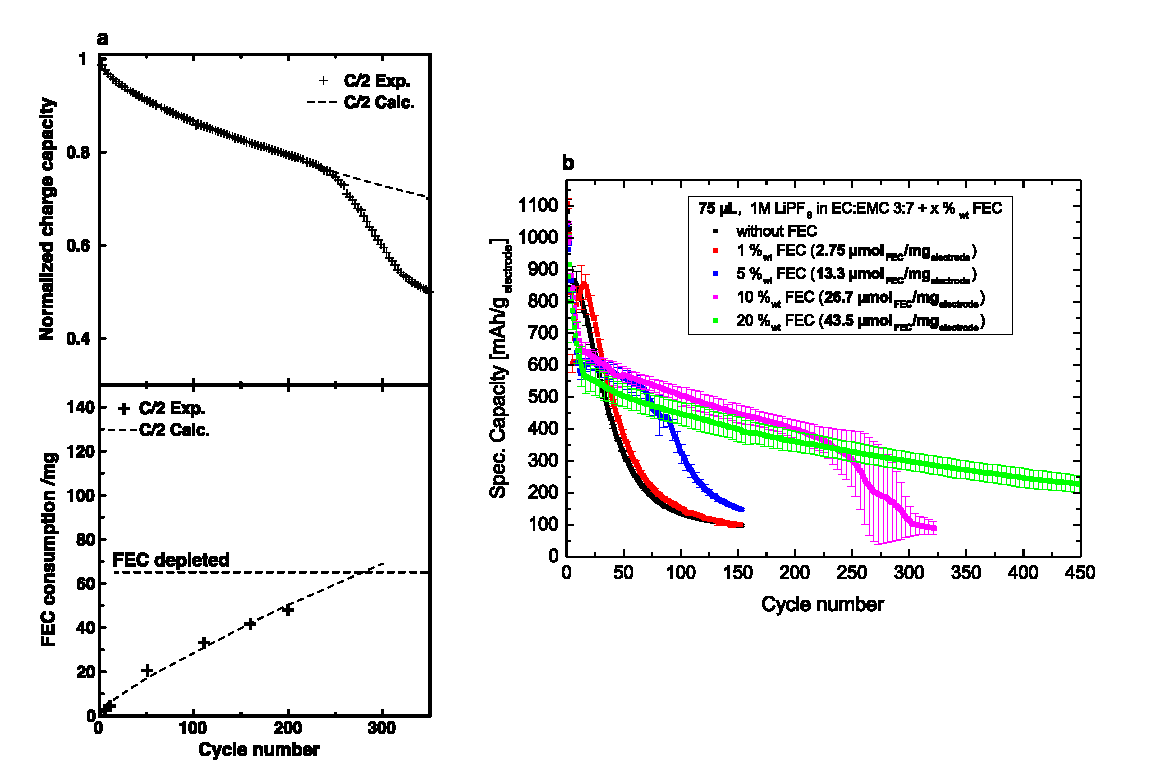
\includegraphics[scale = 0.7]{figures/fec_depletion.eps}
\caption{Additive depletion knees.
(a) The capacity retention of a full cell with 15\% Si in the negative electrode exhibits a knee at around 250 cycles, the same point at which the FEC is depleted from the electrolyte (from destructive gas chromatography-mass spectrometry measurements of FEC concentration). Adapted from Figure 8 of Petibon et al.\cite{petibon_studies_2016}
(b) In half cells with 100\% Si negative electrodes, the cycle number of the knee increases with the FEC concentration in the electrolyte. Adapted from Figure 1 of Jung et al.al.\cite{jung_consumption_2016}}
\label{fig:fec_knee}
\end{figure}

This knee pathway has a number of interesting implications.
First, since laboratory-built cells are often filled with high electrolyte volumes, knee mechanisms that are not present in lab testing may manifest in more commercially representative form factors.
As Wetjen et al.\cite{wetjen_differentiating_2017} emphasize,
maintaining representative electrolyte volumes in lab-scale cells is critical for accurately capturing this knee pathway in production-scale cells.
Second, nominally identical cells, cycled identically, but with different initial FEC concentrations exhibited minute electrochemical differences before the knee.\cite{jung_consumption_2016}
Theoretically, only the FEC consumed in a given cycle manifests in the electrochemical signals from cycling (e.g., differential capacity or differnetial voltage analysis); the excess FEC is not electrochemically detectable as it does not participate in reactions with the electrode.
Since the \emph{remaining} FEC amount is the main determinant of cycle life in these cells, the knee point of cells exhibiting this mechanism is not predictable via standard electrochemical signals.
An interesting proposal for future work is to evaluate other nondestructive probes (e.g., acoustic signals\cite{knehr_understanding_2018}) that may be sensitive to FEC concentration in the electrolyte.

\subsection{Electrode/electrolyte connectivity}

\pbox{
Looks great, just need to complete
}

[Edwin: I will write a brief introduction to percolation theory to start this section. Then, I will talk about how percolation theory is used in electrolyte dry-out and electronic connectivity. This would be a threshold type of knee where the threshold is the critical ``saturation'' (Fig. 5 in Kupper et al.'s paper).]

Percolation theory (cite Essam and Stauffer and Aharony) is commonly used to describe statistical properties of clusters that are geometrically connected in porous media such as porous electrodes used in modern lithium-ion batteries. A general characteristic of a system described by percolation theory is the existence of a critical threshold above which the probability of a spanning cluster being formed tends towards one and below which this probability tends towards zero.

Kupper et al.~\cite{kupper_end--life_2018} model what they call ``sudden death'', i.e., knee, by introducing a percolation threshold in the activity-saturation relationship, which is linked to electrolyte dry-out. This percolation behavior of the liquid electrolyte is similar, but not identical, to the one studied for ``effective diffusive conductivity`` and tortuosity by Ferguson and Bazant~\cite{ferguson_nonequilibrium_2012}.

[Edwin: We will need to state the definitions of activity and saturation used by Kupper et al. since they are non-standard.]

The activity $a$ and liquid saturation $s$ are given by
\begin{align}
    a &= \frac{\varepsilon_{\text{LiC}_6}}{\varepsilon_{\text{LiC}_6,\text{inactive}}+\varepsilon_{\text{LiC}_6}}, \quad s = \frac{\varepsilon_\text{elyt}}{\varepsilon_\text{elyt}+\varepsilon_\text{gas}}.
\end{align}
The two nonlinear relationships used to model percolation behavior of the liquid electrolyte are given by
\begin{align}
    a &= 0.5\tanh\left(10\left(s-0.5\right)\right) + 0.5, \\
    a &= \left(0.5s+0.5\right)\left(0.5\tanh\left(15\left(s-0.4\right)\right)+0.5\right),
\end{align}
which correspond to Relationships 3 and 4 respectively in Figure~\ref{fig:activity-saturation-relationships}.

[Edwin: We can reuse (after asking for permission) Fig. 5 in Kupper et al.'s paper and Fig. 10 in Ferguson's paper here to illustrate the percolation threshold.]

\begin{figure}[ht]
\centering
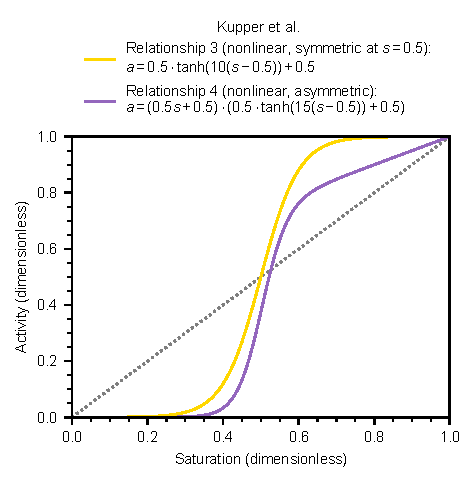
\includegraphics[scale=1.0]{figures/percolation.eps}
\caption{Activity-saturation relationships adapted from Figure 5 of Kupper et al.\cite{kupper_end--life_2018} Relationships 3 and 4 model percolation of the liquid electrolyte.}
\label{fig:percolation}
\end{figure}

\begin{figure}[ht]
    \centering
    \includegraphics[scale=0.75]{figures/A3468fig5.jpeg}
    \caption{Activity-saturation relationships taken from Figure 5 of~\cite{kupper_end--life_2018}. Relationships 3 and 4 are nonlinear and model percolation of the liquid electrolyte.}
    \label{fig:activity-saturation-relationships}
\end{figure}

Electronic connectivity: Li et al.~\cite{li_effects_2015}.

Distinct from LAM causing plating, as this can cause a knee in its own right.

Although Kupper et al.'s work did not provide a convincing experimental validation to demonstrate that electrolyte dry-out results in the proposed loss of liquid electrolyte percolation, it is plausible and should be studied in more detail in the future. 

\subsection{Mechanical degradation}

Mechanical degradation can be split into macroscale effects occurring at the cell scale and microscale effects occurring at the particle scale.

\begin{figure}[ht]
\centering
\includegraphics[scale = 0.7]{figures/MechanicalKneepoints.pdf}
\caption{Knee point occurrence linked mechanical effects: With cycles particles and the SEI expand and crack leading to the formation and regrowth of additional SEI. In addition a covering layer was found forming on the anode surface. Pressure due to volume expansion can also lead to jelly roll deformation in cylindrical wound cells. This can induce delamaniation and loss of active material leading to more SEI and covering layer growth. (Philipp -- looks great, please add caption)}
\label{fig:knee_mechanical}
\end{figure}

\paragraph{Macro scale mechanical effects.}

High stack pressure can cause knee. High mechanical stress is not evenly distributed throughout the inside of the pouch, causing heterogeneous delamination, surface film formation, and uneven lithium distribution. LAM attributed to anode from half-cell data, no change in LAM PE. Similar to temperature there is a sweet spot for stack pressure\cite{cannarella_stress_2014}. The stack pressure can be set and measured in pouch cells \cite{wunsch_investigation_2019} and prismatic cells\cite{cannarella_stress_2014}, but  with cylindrical cells only measured\cite{willenberg_high-precision_2020}

Depending on the type of bracing, the pressure over the lifetime evolves differently . Wünsch et al. \cite{wunsch_investigation_2019} reported a thickness increase for unbraced cells correlated with knee point. They also showed with the right bracing, for example deforming elements on both sides of the cells, the lifetime could be increased from 500 to 3200 cycles.
Another effect was found with CT studies on 18650s revealing jelly roll deformation, Pfrang et al. \cite{pfrang_long-term_2018} using cells from Ecker et al. \cite{ecker_calendar_2014}
From post-mortem analysis Bach et al. could show a link between heterogenous pressure and uneven ageing and plating\cite{bach_nonlinear_2016}.

The effects discussed here are inherently multidimensional (at the macroscale) in nature and hence cannot be captured by standard electrochemical models, which are one-dimensional at the macroscale. Instead, they would require complex three-dimensional models, whose computational complexity is prohibitively high for simulating degradation over hundreds of cycles. We are not aware of any current modeling efforts in this direction [right?]. One reduced-order modeling approach could be to couple one-dimensional electrochemical models with network models for the jellyroll \cite{tranter_probing_2020}.  Another possible modeling approach is to use homogenization methods on the jellyroll \cite{psaltis_homogenisation_2020} to elucidate the mechanical behavior (and buckling) of the spirally-wound layers.

\paragraph{Micro scale mechanical effects.}


\pbox{
Add covering layer stuff
}

At the microscale, repeated intercalation/de-intercalation causes stress in the particles that can then lead to loss of active material through particle cracking.
Reniers et al.~\cite{reniers_review_2019} show that there can be a positive feedback between the stress and the loss of active material leading to a (snowballing) knee point. They model this using a fatigue model for loss of active material due to stress from Laresgoiti et al.~\cite{laresgoiti_modeling_2015} with a stress model from Dai et al.~\cite{dai_simulation_2014}: higher stress causes higher LAM, which in turn increases the current density and hence causes higher stress.

Lin et al.~\cite{lin_comprehensive_2013} propose a different mechanism for knee points caused by loss of active material. In their model, SEI formation leads to loss of lithium inventory and mechanical effects in the cathode lead to LAM. This causes the the cathode utilization to increase and shift to a steeper open-circuit potential, which reduces the capacity between voltage limits. This mechanism produces a non-linear capacity fade (knee point), due to the non-linearity of the open-circuit potential, despite linear LAM and self-limiting SEI formation. The knee point occurs when loss of active material outpaces loss of lithium inventory, as suggested by Dubarry et al.~\cite{dubarry_durability_2018}.

Other authors have suggested that mechanical effects can accelerate SEI growth by causing SEI cracking and revealing new active surface area to grow \cite{kupper_end--life_2018,louli_operando_2019}. Since SEI formation is still self-limiting, this effect alone is not enough to lead to a knee point, but it could accelerate the onset of knee points in other mechanisms related to SEI formation.
In addition to SEI formation, covering layers on the anode surface were reported on cells with knee points \cite{lewerenz_post-mortem_2017,willenberg_development_2020,stiaszny_electrochemical_2014}. These layers were also characterized as passivating or dead lithium agglomerates \cite{schindler_fast_2018}.

\pdebox{
Figure with post-mortem pictures included here, but needs to condensed. Can be found in Google slides
}

% Rainflow model for stress in batteries: Xinran Xiao (Michigan State), Deshpande battery fatigue
% Nice figures for this in Kupper 2018, Louli 2019.

\section{Factors influencing the knee}

We surveyed the literature to identify empirical case studies in which the knee point can be controlled via changes to a single variable. Table S1 classifies these case studies into three categories based on the nature of the variable: cell design, testing conditions, and sampling/testing variability (a special case of these two categories). Some testing conditions have a consistent impact on the emergence of the knee; for example, higher charging rates and wider cycling voltage ranges accelerate the appearance of the knee. However, the impact of other variables (e.g., discharging rate and rest times) is less clear and may depend on the specific cell design and operating conditions.

\subsection{Cell design}

While the dependence of knees on cell usage conditions has been the focus of much previous work, less attention has been focused on the dependence of knees on cell design---likely due to the challenges of lab-scale cell fabrication. Perhaps the most comprehensive references on this topic come from the Dahn lab. Specifically, Ma et al.\cite{ma_editors_2019} studied the impact of various electrodes and electrolytes on the location of the knee, finding that cathode particle coatings and low cathode loadings delayed the knee location. These knees were classified as DCR ``pseudo-knees'' due to increased electrolyte oxidation on the cathode, as evidenced by the strong dependence of the knee severity on discharge rate as well as cathode impedance measurements. Ma et al. al.\cite{ma_editors_2019} and Glazier et al.\cite{glazier_analysis_2017} also found that the graphite type (i.e., natural or artificial) substantially impacts the knee location, though the root cause of the knee in this case is unclear(PETER TO EXPLORE FURTHER).

Electrode loadings---specifically, anode loadings---can also lead to knees via the lithium plating pathway.
If the electrode is too thin/capacity is too low, thermodynamic plating can occur; however, kinetic plating can occur if the electrode is too thick. (LI PLATING TEAM--WHAT ARE GOOD REFERENCES FOR THESE?)

Additionally, small changes in the electrolyte can play an outsized role on the lifetime performance. Ma et al.\cite{ma_editors_2019} demonstrated the sensitivity of the knee location to the electrolyte additive package; specifically, high methyl acetate (MA) concentrations (MA is used to increase electrolyte transport capability) and low LiPF$_6$ concentrations consistently lead to earlier knees. These knees were attributed to increased electrolyte oxidation on the cathode. Ma et al.\cite{ma_editors_2019} also identified other electrolyte systems with a strong knee sensitivity. Additionally, as previously discussed, additive depletion (e.g., FEC depletion in cells with high silicon content in the anode) can be a direct cause of knees for some cell designs.

Lastly, mechanical deformation knees are naturally highly sensitive to the cell form factor. For instance, deformation of the core(PHILIPP -- WHAT PAPERS TO CITE?) can only occur in cells with cores, namely cylindrical cells.

\subsection{Testing conditions}

\subsubsection{Charging rate}
Increasing the charging rate has accelerated the onset of the knee-point across a range of batteries. \cite{lewerenz_systematic_2017,lewerenz_post-mortem_2017, petzl_lithium_2015, burns_-situ_2015, waldmann_optimization_2015, schuster_nonlinear_2015, severson_data-driven_2019, schindler_fast_2018, keil_linear_2019}. However, the critical charging rate leading to knee-onset varies substantially, with knees appearing at C-rates as low as 1C \cite{waldmann_optimization_2015} and as high as 8C \cite{lewerenz_systematic_2017}. 

Higher charging rates advance the knee point via Li plating and accelerated SEI growth. Either Li plating or SEI growth may directly cause knee onset, but knee onset is also attributed to pore clogging caused by either or both of these mechanisms \cite{yang_modeling_2017}. It is difficult to distinguish these causes, even in cases with detailed post-mortem characterization. Key evidence for both Li plating and accelerated SEI growth driven by increased charging rate is found in a series of papers by Lewerenz et. al., examining the aging of cylindrical 8 Ah LFP/Gr cells \cite{lewerenz_systematic_2017,lewerenz_post-mortem_2017}. They present evidence demonstrating that knees reliably occur across a set of test replicates at 8C charging rate, while knees may occur less reliably at charging rates as low as 2C. Evidence of Li plating after knee onset driven by increased charging rate was also confirmed by Petzl et. al. \cite{petzl_lithium_2015} and Burns et. al. \cite{burns_-situ_2015}. 



\subsubsection{Discharging rate}

Unlike charging rate, the effect of discharging rate on the knee point is mixed (Figure X).
In some systems, an increased discharging rate
accelerates the knee onset.
Omar et al.\cite{omar_lithium_2014} found that a higher discharging rate (1C to 15C) accelerated the knee for cylindrical LFP/graphite cells.
Diao et al.\cite{diao_accelerated_2019} showed no effect of discharge rate except at 60°C, where the cells discharged at 2C degraded almost twice as quickly than the cells discharged at 0.7C or 1C.
High discharging rates can lead to worse cycle life due to higher temperature, which accelerates electrolyte reduction (i.e., SEI growth) and electrolyte oxidation (i.e., cathode resistance growth). Additionally, high discharging rates can lead to ``pseudo-knees'' when the resistance growth or lower cutoff voltage is high.

In other systems, an increased discharging rate can delay the onset of the knee.
Atalay et al.\cite{atalay_theory_2020} found that reducing the discharge rate from 4C to 1C accelerated the knee for 18650 NCA/graphite cells.
Keil et al.\cite{keil_charging_2016} illustrated how discharging current had no effect on LMO+NMC/graphite and LCO+NCM/graphite cylindrical cells, but a lower discharging current (3A, 2.7C) lead to faster degradation than a higher discharging current (5A, 4.5C) for an LFP/graphite cylindrical cell when charged at 4.5C; they did not identify a mechanism. 
Similarly, Keil et al.\cite{keil_linear_2019} found that increasing discharging current from 1C to 2C lead to the elimination of the knee in NMC/graphite cylindrical cells.
While more work is needed to understand these results, one hypothesis for these observations is increased calendar aging for cells with faster discharge rates.
In other words, cells with less time spent cycling simply have less calendar aging. This hypothesis does suggest a sensitivity of the x axis to the apparent severity of the knee; for instance, plotting retention vs. time instead of cycle number may decrease the apparent severity of the knee.

\subsubsection{Voltage limits} 
A wider voltage window generally accelerates the onset of the knee point \cite{ecker_calendar_2014, pfrang_long-term_2018, klett_non-uniform_2014, ma_novel_2019, petzl_lithium_2015, schuster_nonlinear_2015}. In one of the broadest studies, Ecker et al. \cite{ecker_calendar_2014} considered six DODs (100, 80, 50, 20, 10, and 0.5 \%) with up to six voltage windows per DOD. They found that the EFC systematically decreased with increased DOD. By 1000 EFC, all cells with DODs greater than 25-75 \% had a capacity below 80 \% and showed a knee point. When varying the voltage window at the same DOD, the authors observed the highest degradation in cells cycled at low and high SOCs; the lowest degradation was observed for a midpoint SOC of 50 \%. Accelerated degradation at extreme SOCs was also observed in other studies \cite{aiken_accelerated_2020,ma_novel_2019, zhu_investigation_2021}.

The impact of the voltage window on knee point onset is typically attributed to DCR growth stemming from enhanced expansion and cracking of the electrode during intercalation. In several studies, capacity knees have aligned perfectly with resistance knees \cite{ecker_calendar_2014, klett_non-uniform_2014, schuster_nonlinear_2015, zhu_investigation_2021}. High voltages may also drive electrolyte oxidation at the cathode \cite{aiken_accelerated_2020} and for some cathodes, active material loss via Mn dissolution \cite{ma_novel_2019}. 



\subsubsection{Rests (Peter to finish)}

The effect of rests during cycling is mixed. 
Keil et al.\cite{keil_linear_2019} found that decreasing rest time at both TOC and BOD from 900s to 10s delayed the knee point in graphite/NMC cylidrical cells.
Ma et al.\cite{ma_editors_2019} found an identical result: removing the 30 min rests at both top-of-charge and bottom-of-discharge delayed the knee, but only with an upper cutoff voltage of 4.3 V. The rest time had no effect at 4.1 V.
These observations were rationalized by less time at high potential when plotted as a function of cycle number.

In contrast, Epding et al.\cite{epding_investigation_2019} found that longer rest times in between rounds of cycling helped. This rest offered reversibly plated Li time to reintercalate.

Depends on if cycling typically or with plating.

This paper (not in overleaf yet) could support why increased rests are good:

%https://web.iitd.ac.in/~agupta/Papers/Rashid_Gupta_JECS2015.pdf 

\subsubsection{Temperature}
The effect of temperature on knee onset depends on the test conditions. For example, some studies have found that knee onset is accelerated at temperatures above or below 25 degrees Celsius \cite{zhang_accelerated_2019, waldmann_temperature_2014, waldmann_optimization_2015} or 35 degrees Celsius \cite{schuster_nonlinear_2015}. In general, the temperature of minimal degradation is lower for LFP cells than NMC cells \cite{SNL long-term cycling paper}. 

There is no straightforward dependence on temperature because different mechanisms dominate in different temperature ranges (Figure Waldmann temperature V). At lower temperatures, the acceleration of the knee point is attributed to Li plating. At elevated temperatures, knee point onset is driven by SEI growth \cite {zhang_accelerated_2019,schuster_nonlinear_2015,waldmann_temperature_2014,waldmann_optimization_2015}.

\subsubsection{Pressure}
Studies of pressure dependence in pouch and prismatic cells have demonstrated 'sweet spots' for optimal performance. The knee point can be accelerated by either an absence of pressure or excess pressure. For example, Wünsch et al. increased the cycle life of 37 Ah commercial NMC pouch cells from 500 (no bracing) to 3200 (optimal spring compression) while investigating various methods of bracing \cite{wunsch_investigation_2019}. Figure xyz shows another example from Cannarella et al. for an LCO pouch cell \cite{cannarella_stress_2014}. Even in a cylindrical cell, heterogeneous compression in the test fixture can accelerate the knee point \cite{bach_nonlinear_2016}. 

For pouch and prismatic cells, some applied pressure is needed to enhance conductivity and particle contact. When too much pressure is applied, high mechanical stress is not always evenly distributed throughout the cell. This causes heterogeneous delamination, surface film formation, and uneven Li distribution (Li plating). Li plating was also reported in cylindrical cells that experienced heterogeneous compression from test fixtures \cite{bach_nonlinear_2016}. 



\subsection{Sampling and testing variability}

Nominally identical cells cycled identically often show differences in knee behavior. This sampling variability includes both intrinsic variability from manufacturing (component-level variation, cell assembly, etc) and extrinsic variability from testing (cycler calibration, temperature control, etc). These sources of variability cannot be distinguished.

The magnitude of sampling variability is a function of the cell design, manufacturing variability, and testing conditions. Sampling variability may increase with more aggressive cell designs, more manual cell assembly processes, and more aggressive testing conditions (particularly for test setups with no or poor temperature control). The magnitude of sampling variability can be estimated using studies with fairly large sample sizes (i.e., at least $\sim$10 cells). Baumhöfer et al.\cite{baumhofer_production_2014} and Harris et al.\cite{harris_failure_2017} studied this type of variation in 48 cells and 24 cells, respectively, finding widely varying knee locations across their datasets. Note that these studies did not identify a correlation between beginning-of-life capacity and end-of-life capacity, suggesting that the underlying state variables controlling the knee location did not manifest in the initial capacity measurements. In general, sampling and testing variation also poses challenges for accurate knee prediction; we recommend identifying the manufacturing and testing variation of the state variable of interest in evaluating the accuracy of knee prediction methods. Beck et al.[CITE] provide a detailed review of cell-to-cell variation.

\section{Predicting knees}

\pbox{Anyone interested? I think a key message here is which pathways/types of pathways can be predicted theoretically and with measurements}
\newline
\ssri{I think this would be really valuable because predicting knees is really the economic value addition from all the knee point analysis. We spoke a little bit about how ML could predict knees -- given how much we've talked about pathways (also as mentioned by Peter above), I think there is a point to be made about physics-inspired/physics informed ML i.e., an ML framework coupled with an electrochem model which is one of the few ways in which something about the pathways can also be said in addition to the ML predicted knee. Goes a long way in making falsifiable ML models wrt knees.}

\subsection{Relationship between knees and end-of-life}

While predicting knees is important, predicting end-of-life is more directly relevant for product performance and estimating warranty costs. Thus, we explored the relationship between knee locations and end-of-life.

\begin{figure}[ht]
\centering
% \begin{subfigure}{.5\textwidth}
%   \centering
\includegraphics[width=0.8\linewidth]{figures/AcrossDatasetsknee-to-EOL}
%   \caption{Linear regression of knee-point to EOL point}
  \label{fig:kneepoint2EOL}
% \end{subfigure}%
\caption{Total of 306 cells across 15 datasets. The knee identification algorithm employed is the Bacon-Watts one. Linear relation between knee-point and EOL (defined as 80\% capacity).}
\label{fig:knees2EOL}
\end{figure}

\subsection{Prediction outlook}

Figure \ref{fig:snowball_vs_hidden_vs_threshold} illustrates three types of underlying mechanisms.

\pbox{My takeaways so far:
\begin{itemize}
    \item Snowballs will be hard to extrapolate
    \item Challenge is identifying the right state variable to track, and actually tracking it
    \item Some state variables are ``electrochemically invisible'', e.g. remaining FEC content in the electrolyte.
    \item Multiscale modeling needed (SEI growth/cathode DCR growth, electrode porosity/connnectivity changes, macroscale mechanical deformation)
    \item need for low rate cycling
    \item In the field vs lab testing
    \item Online estimation 
    \item Pulse measurements. Superlinear increase in resistance is bad news
\end{itemize}
}

Goncalo: Can the mechanism be predicted from the data?

\section{Conclusions and future work}

Knees are a major challenge to developing long-lasting lithium-ion batteries. In this work, we first evaluated definitions of knees and identified three different types of underlying mechanisms leading to a knee, each with different implications for knee prediction. We then critically investigated the literature support for (five/six) knee pathways, including lithium plating, resistance growth, additive depletion, percolation-limited connectivity, and mechanical deformation.

\section{Supporting Information}

Table S1. Summary of experimental variables leading to knee points


Yuliya: See table in Excel document tab 'SI-Exp Tables'. 


Table S2 classifies previous efforts to model the knee point as physics-based, equivalent circuit, or empirical. [add explanation of table columns]

Table S2. Summary of previous knee point modeling efforts

\bibliographystyle{myIEEEtran}
\bibliography{refs_zotero}




\end{document}
